
\section{Arquitectura}

% Documento que describa las principales decisiones de arquitectura que fueron evaluadas y la decisión que se tomó en cada caso. Se deberá incluir una o más vistas que describan la visión general de cómo será el producto en el nivel de la arquitectura.

\subsection{Vista principal de componentes y conectores}

\begin{figure}[H]
\centering
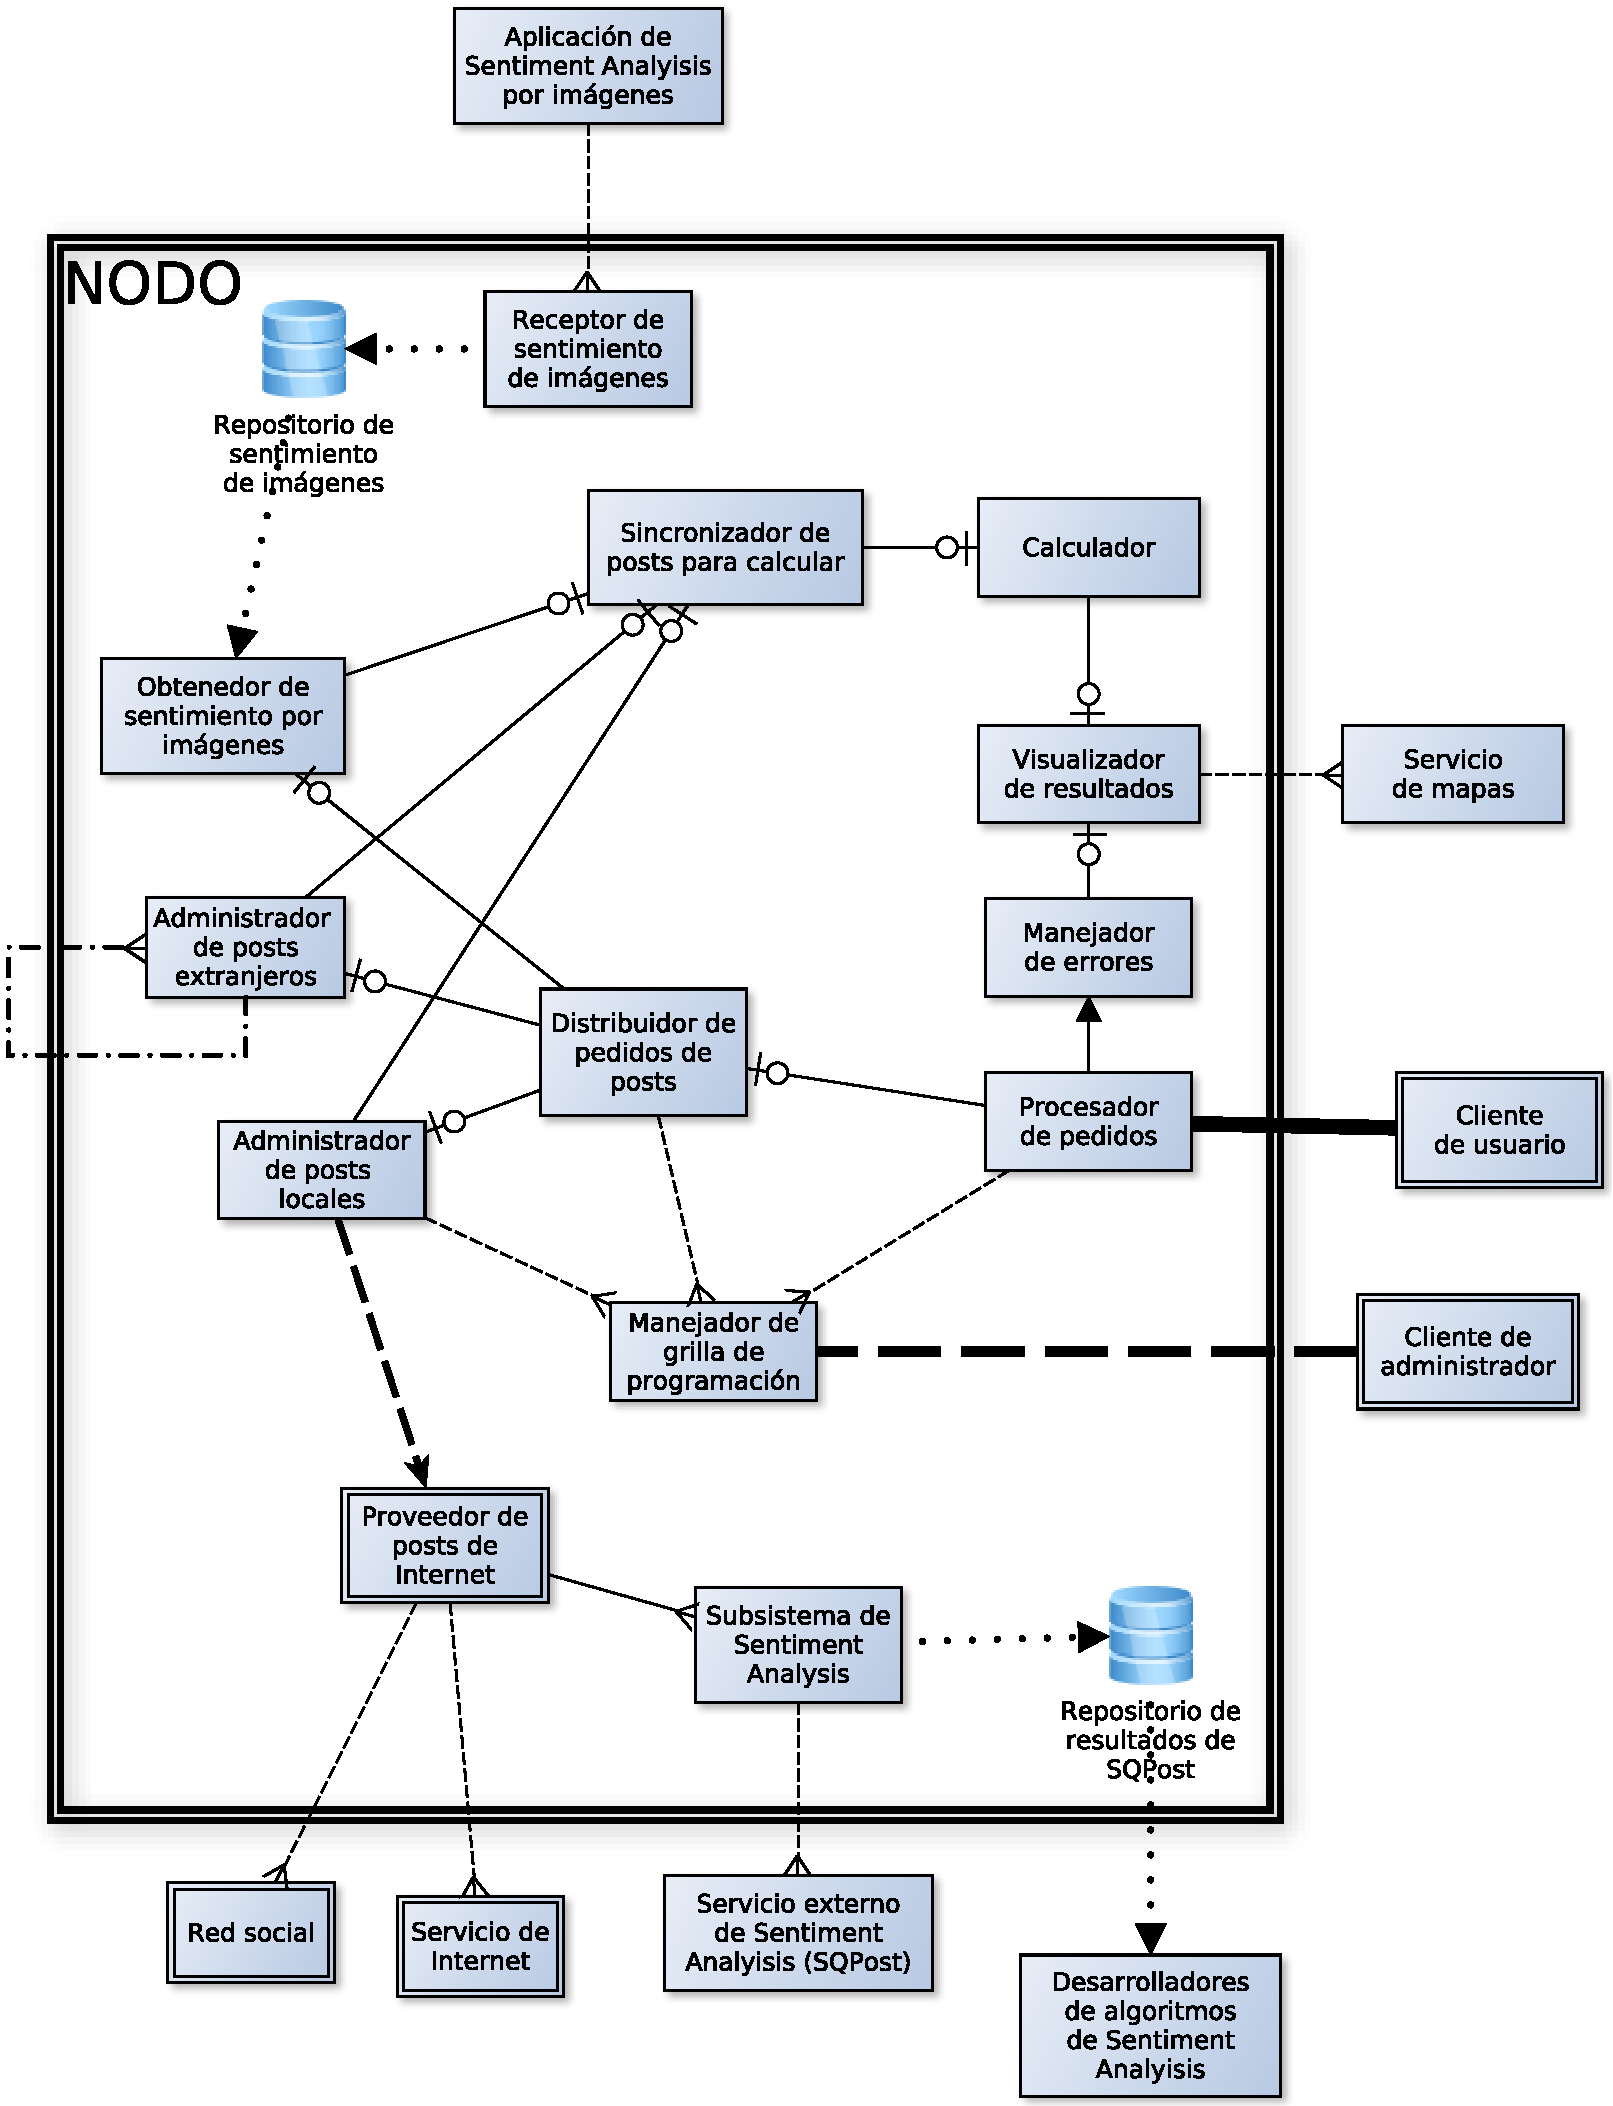
\includegraphics[width=\textwidth]{graph/main.pdf}
%\caption{Post Filterer}
\end{figure}

\begin{figure}[H]
\centering
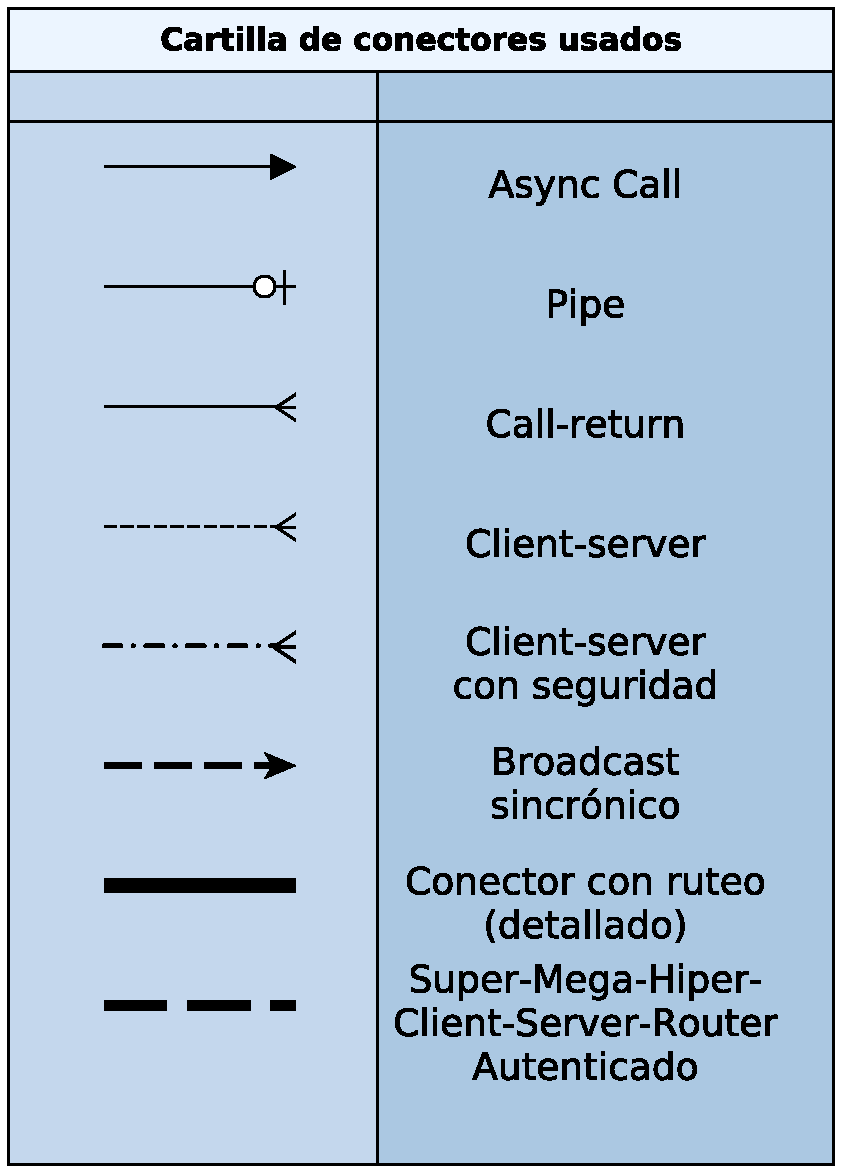
\includegraphics[width=0.5\textwidth]{graph/cartilla.pdf}
%\caption{Post Filterer}
\end{figure}


\subsection{Conector que rutea pedidos}

\begin{figure}[H]
\centering
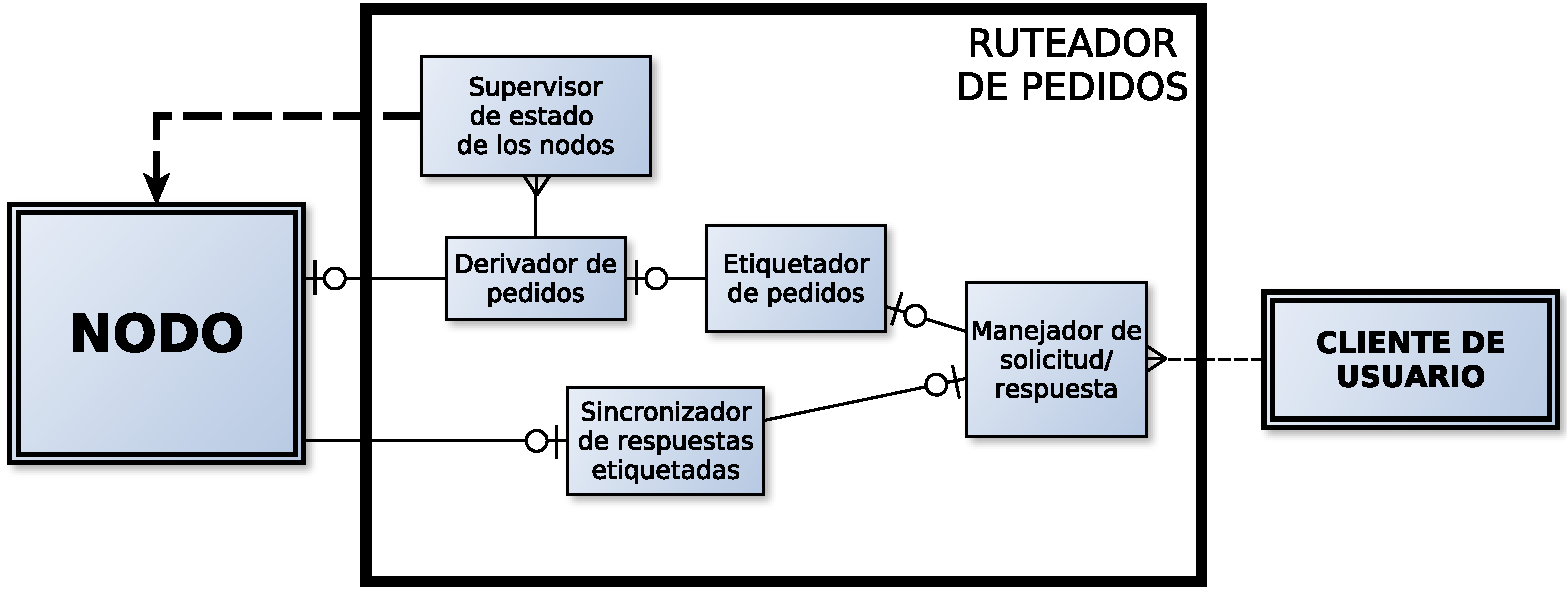
\includegraphics[width=\textwidth]{graph/conector.pdf}
%\caption{Post Filterer}
\end{figure}

El cliente se conecta a un servidor web a través de la página de internet del sistema y realiza un pedido. Este pedido debe viajar al nodo más cercano geográficamente a su ubicación. Para esto primero debe pasar por un ruteador de pedidos para que lo diriga.
El pedido llega al manejador, quien mantiene abierta la comunicación con el cliente hasta que llegue la respuesta. El pedido, luego, es etiquetado tal que el resto de los componentes puedan identificarlo a lo largo del flujo de datos. El derivador de pedidos indentifica la IP correspondiente al mismo y la vincula con el nodo al que debería ir. Luego, verifica el estado de dicho nodo y envía el pedido. Si no está activo, entonces, lo envía al siguiente nodo más cercano.

El supervisor de estado es un componente que controla períodicamente si los nodos están activos. Si detecta que algún nodo no responde avisa a los responsables a mediante el envío de un email, para que sea reparado.

Cuando llega la respuesta el sincronizador se encarga de asociarla con el cliente correspondiente utilizando su etiqueta. De esta forma el manejador puede devolver la respuesta al cliente y cerrar la conexión.

Es importante destacar que el ruteador de pedidos está replicado, de manera que siempre que deje de responder puede ser reemplazado inmediatamente y seguir operando. Es vital mantener este componente en funcionamiento ya que sin él no puede realizarse la comunicación con los servidores.

\subsection{Procesador de pedidos}

\begin{figure}[H]
\centering
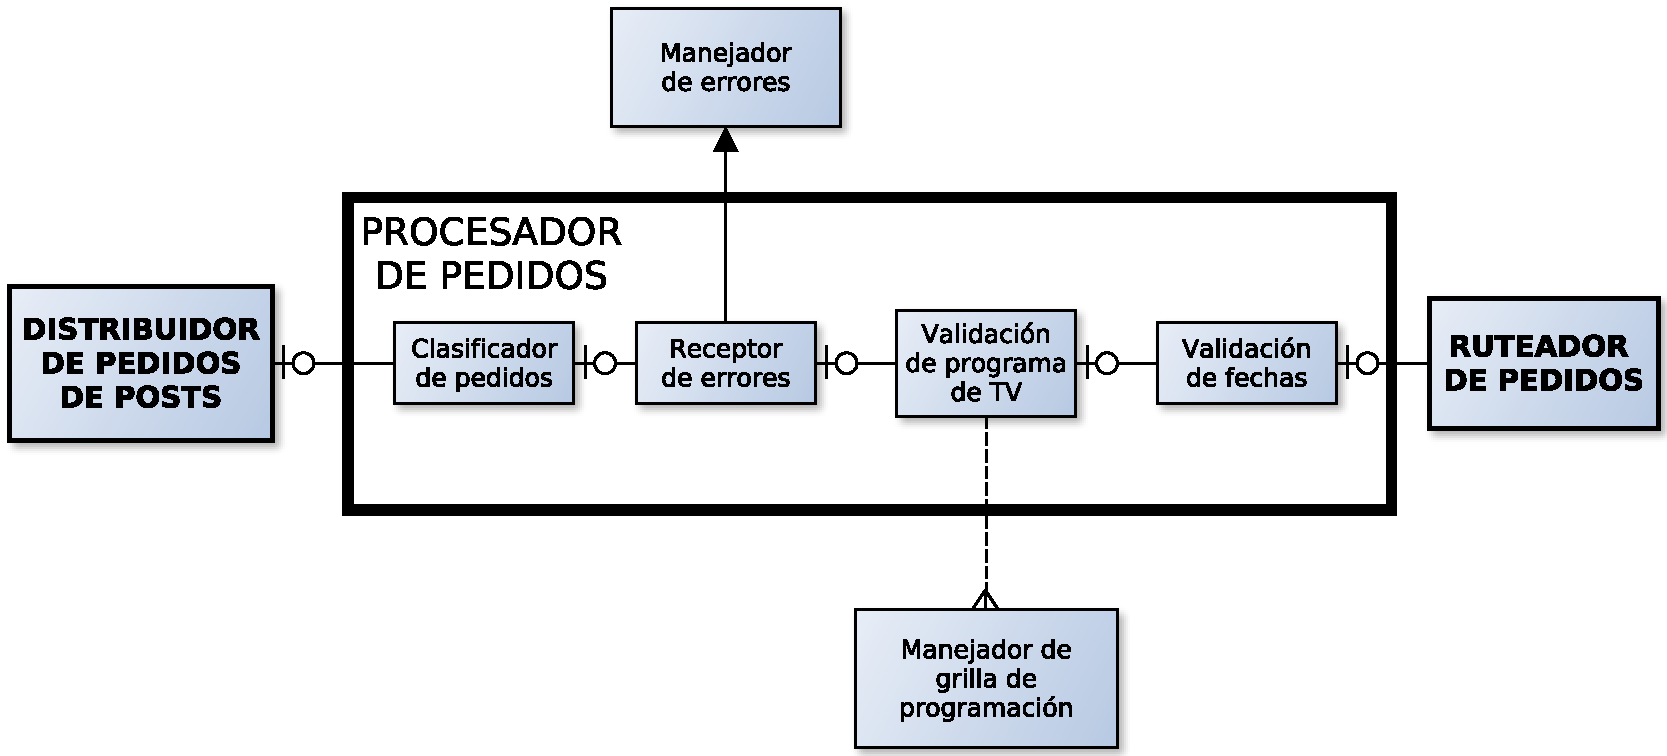
\includegraphics[width=\textwidth]{graph/procpedidos.pdf}
%\caption{Post Filterer}
\end{figure}

Cuando llega un pedido de un usuario de la aplicación al nodo, este componente lo recibe y verifica que las fechas ingresadas tengan un formato válido y que 
además correspondan a un tiempo válido que se pueda consultar. En el caso de que se haya ingresado un intervalo de tiempo, se verifica que este bien constituido (que el inicio sea anterior al final). Luego se verifica que el programa de televisión pedido sea parte de la grilla del sistema, para lo cual se consulta al manejador de la grilla de programación. Si el pedido falla alguno de estos test se envía un mensaje de error que se propaga hasta el receptor de errores quien envía dicho mensaje al manejador de errores para que lo muestre por pantalla. Si el pedido no es filtrado en esta instancia, entonces, pasarña por el clasificador de pedidos que lo etiqueta como pedido de Rating o Popularidad. Una vez hecho esto, se encola el pedido en el distribuidor de pedidos de posts.

\subsection{Distribuidor de pedidos de posts}

\begin{figure}[H]
\centering
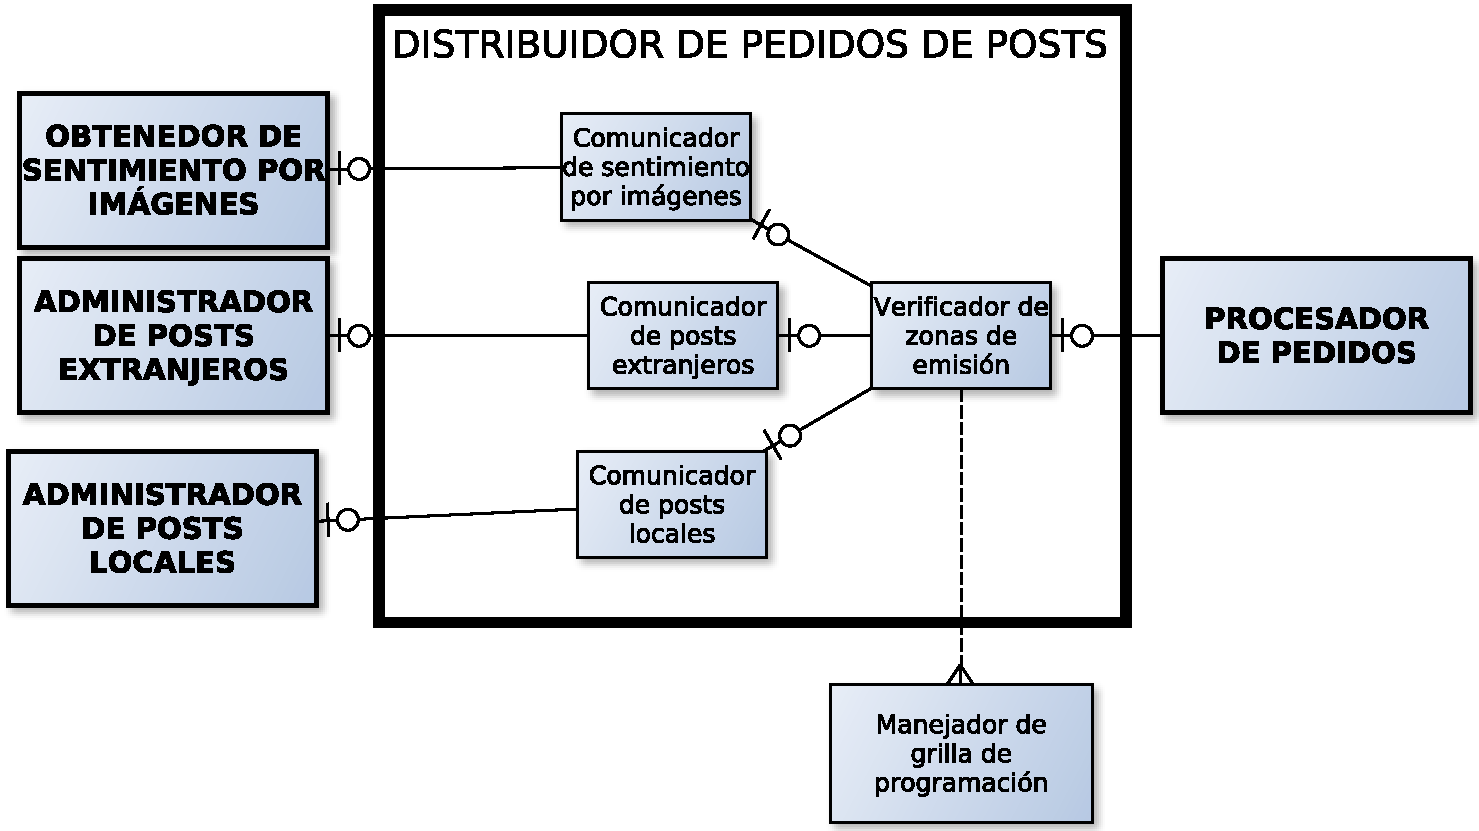
\includegraphics[width=\textwidth]{graph/distribuidor.pdf}
%\caption{Post Filterer}
\end{figure}

Este componente tiene la responsabilidad de pedir los posts necesarios para resolver el pedido del usuario. En primer lugar, se verifica la zona de emisión del programa que fue solicitado para saber si necesita conseguir posts de otras regiones (manejadas por otros nodos) y si necesita posts locales. Se conecta con los comuinicadores para hacer los pedidos correspondientes.

\subsection{Administrador de posts locales}

\begin{figure}[H]
\centering
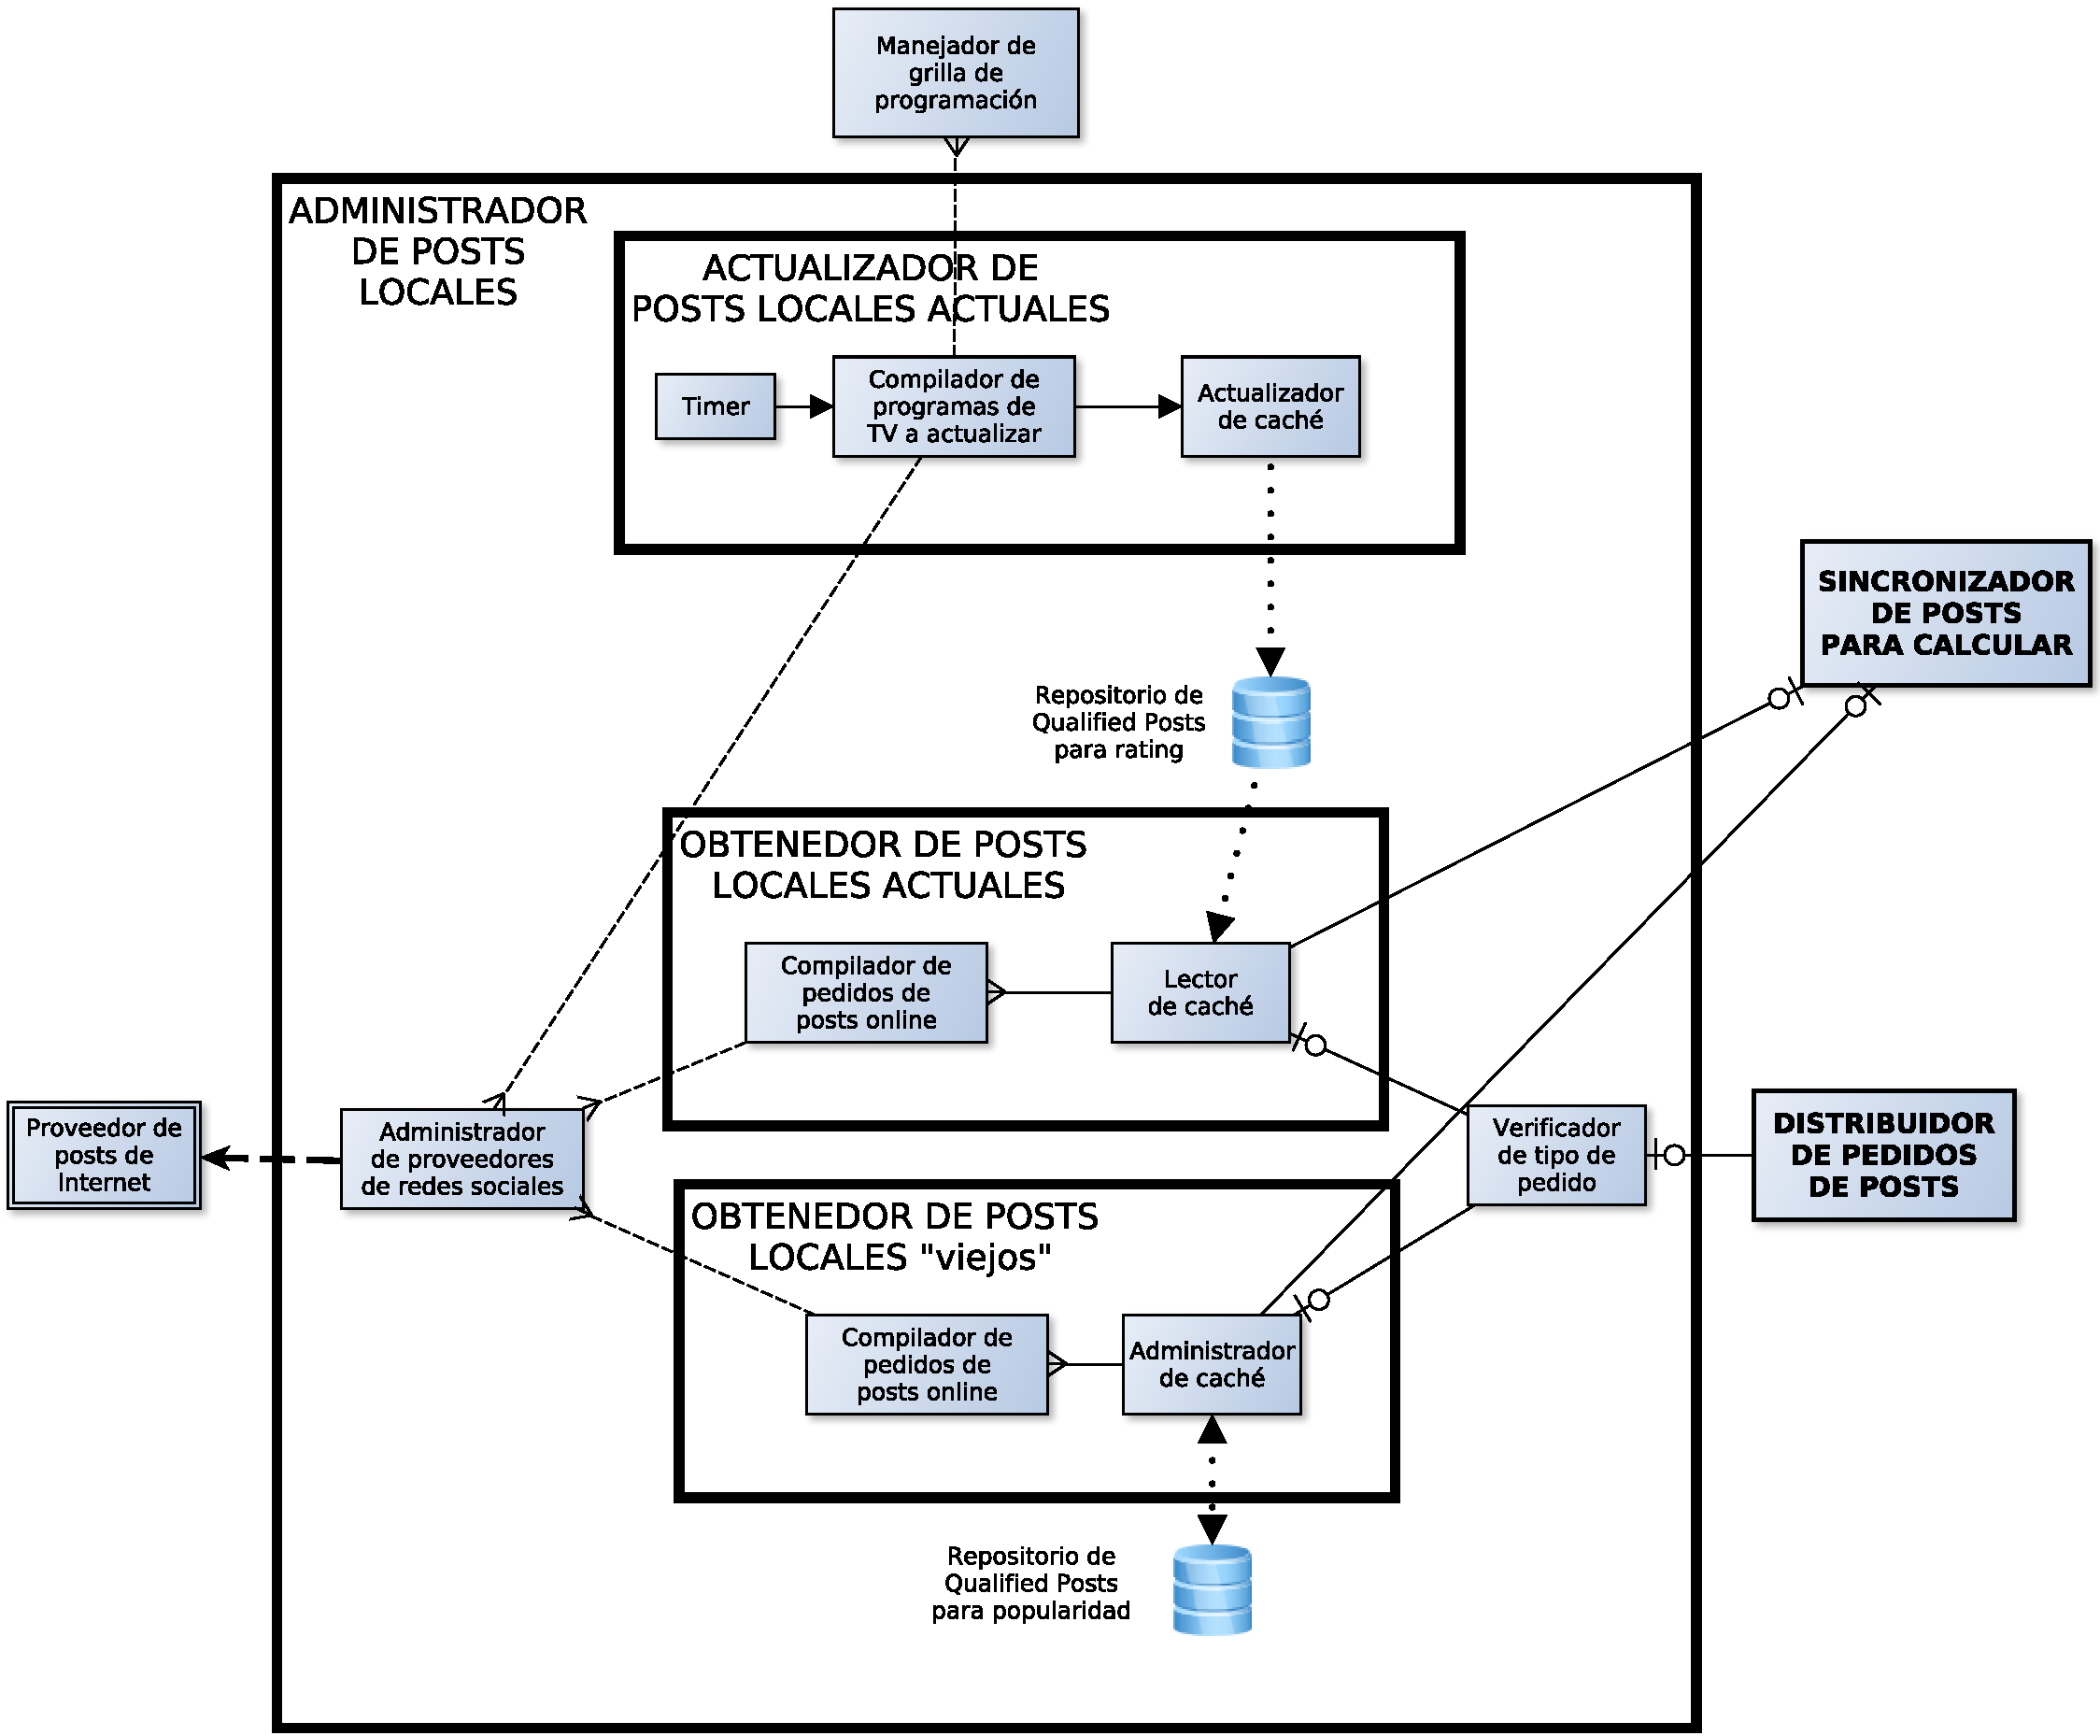
\includegraphics[width=\textwidth]{graph/adminlocal.pdf}
%\caption{Post Filterer}
\end{figure}

Cuando llega un pedido de post a este componente lo primero que se hace es verificar si es un pedido de rating o popularidad. 
Si es un pedido de rating, el obtenedor de post locales actuales revisa la caché correspondiente al ratingpara obtener los posts que necesita, si no los encuentra hace un llamada al compilador de pedidos de posts online. Este organiza el pedido que debe hacerse a las redes sociales y servicios de internet y le envía dicho pedido al administrador de proveedores. Este administrador conoce a cada uno de los proveedores y cada uno de ellos puede conectarse a un determinado sitio de internet. El administrador le pasa el pedido a todos los proveedores. Cada uno de ellos busca en su sitio de internet y responde con qualified posts. Luego, el administrador reune todos los resultados y los devuelve al compilador de pedidos de posts online, que a su vez los devuelve al lector de caché. En este momento el lector caché tiene los resultados del rating correspondientes al nodo local que luego serán sincronizados con los otros resultados.

Si es un pedido de popularidad, se envía al obtenedor de posts locales de popularidad que posee un funcionamiento similar salvo que si recibe datos provenientes de internet las guarda en la cache de popularidad.

Con respecto a la caché del rating, se actualizará constantemente según los programas que esté al aire. La actualización de la caché no depende de los pedidos de rating que se realicen. Es esperable que los pedidos de rating siempre puedan encontrarse en la caché, siempre que esta esté disponible.
La caché de popularidad, en cambio, se actualizará a medida que se realicen pedidos con algún método que priorice las búsquedas más frecuentes. No podemos pretender que los resultados de las búsquedas estén siempre en caché debido a que hay un gran número de consultas posibles, por lo tanto será habitual que para este tipo de pedidos se acceda a las redes sociales. 

\subsection{Subsistema de Sentiment Analyisis}

\begin{figure}[H]
\centering
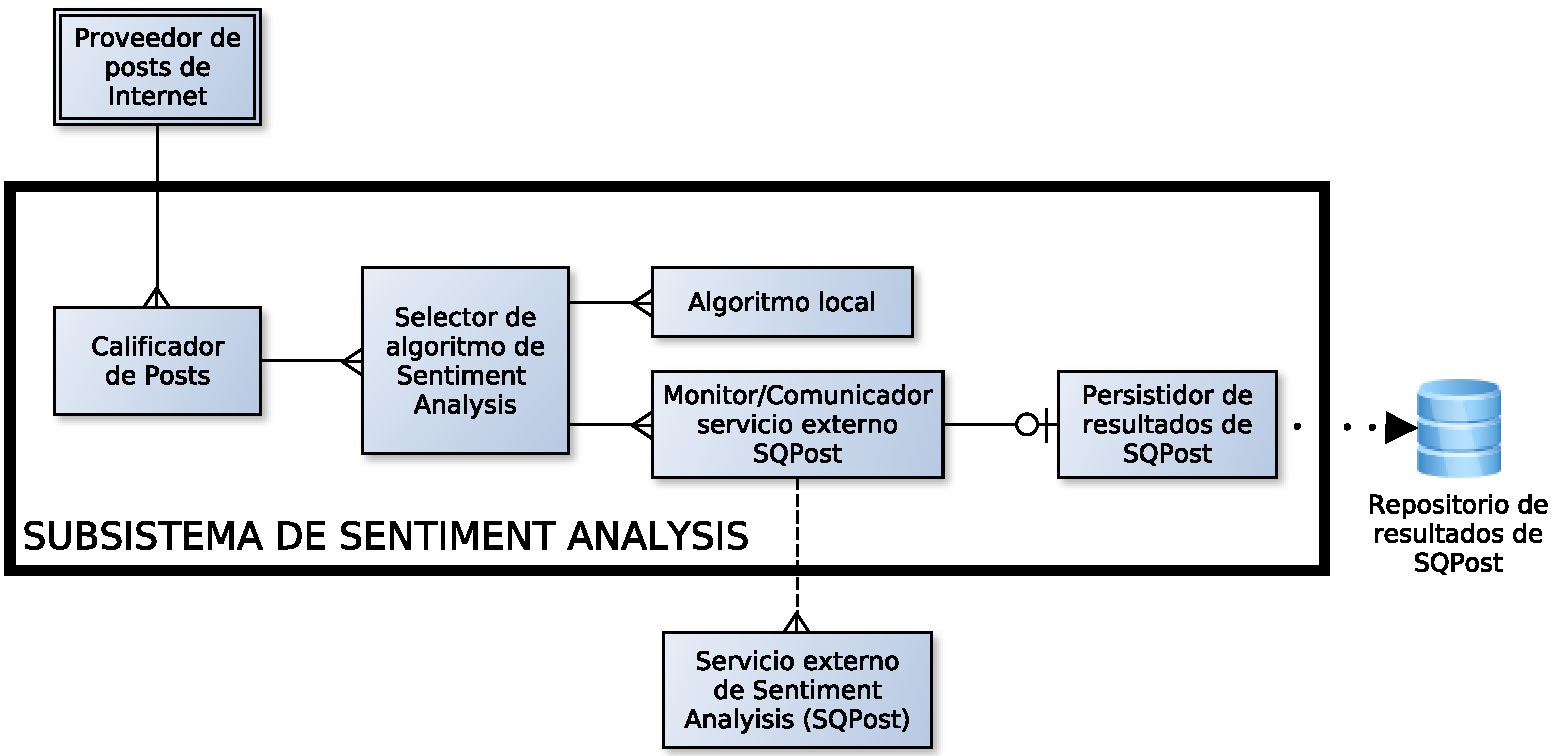
\includegraphics[width=0.8\textwidth]{graph/subsistemaSentimentAnalysis.pdf}
%\caption{Post Filterer}
\end{figure}

El componente de Sentiment Analysis se utiliza para asignarle un sentimiento a cada post que se almacena en el sistema. Cuando un proveedor de posts, vinculado a una determinada red social, obtiene mensajes de dicho sitio y los ingresa al sistema en el formato de post, hace una llamada al Sentiment Analyisis para que los califique. El calificador recibe y organiza los posts, y se conecta con el selector de algoritmo para realizar la calificación propiamente dicha. El selector intenta comunicarse con el servicio externo, que se considera como el más confiable en cuanto a precisión de resultados pero no en disponibilidad. Si recibe una respuesta del servicio, devuelve los sentimientos obtenidos, mientras el persistidor se encarga de almacenarlos en el repositorio para futuros análisis. Si no la recibe, intenta con el algoritmo interno del sistema.

Cuando tiene una respuesta proveniente de alguno de los algoritmos, el calificador convierte los posts obtenidos en posts calificados, y los devuelve para que el proveedor de posts pueda responder la consulta que le habían realizado.


\subsection{Aplicación de Sentiment Analyisis por imágenes}

\begin{figure}[H]
\centering
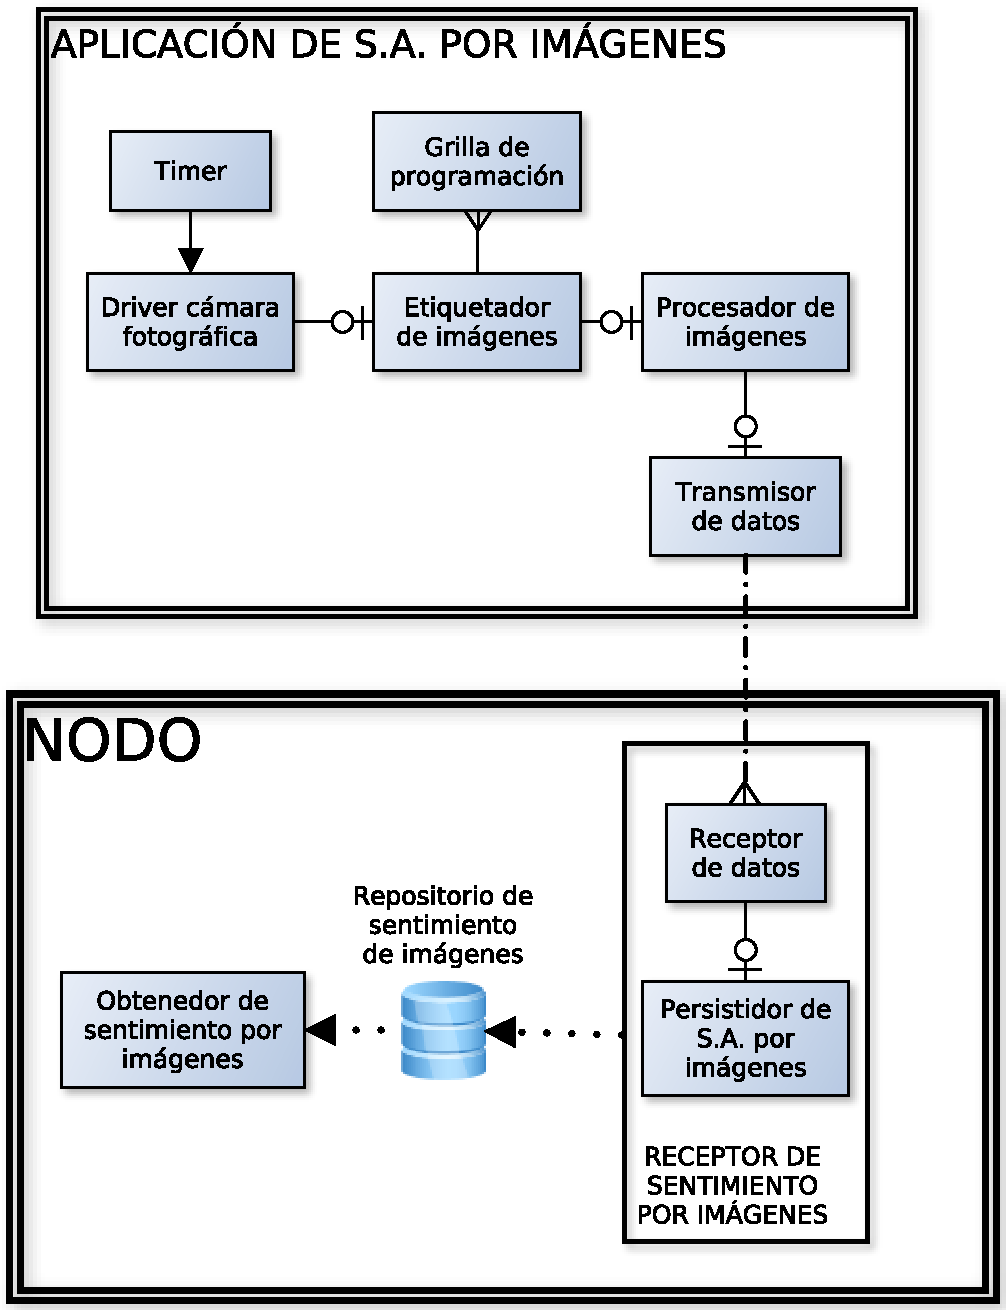
\includegraphics[width=0.7\textwidth]{graph/smarttv.pdf}
%\caption{Post Filterer}
\end{figure}

El sentiment analyisis por imágenes es una funcionalidad del sistema que se agrega a la obtención de datos a través de posts, y ofrece mayor cantidad de datos para operar. La aplicación funcionará en su mayor parte fuera de los nodos, distribuida entre los sistemas de los clientes que ofrecen datos. (Es decir, se ejecutará dentro de los Smart TVs de los usuarios que activen el producto.) El sistema es activado por un timer, que periódicamente indica al driver de la cámara fotográfica del dispositivo que tome una foto y la ponga en cola para procesarla. El procesamiento comienza con el etiquetado de la información, en el cual se le agrega un timestamp y el programa de TV que se está mirando (que un televisor digital puede obtener a partir de la grilla). Luego se procesa la foto en sí, y se obtiene la información de número de personas mirando y datos de cada una, así como su sentimiento respecto del programa de TV.

Los datos anónimos obtenidos de las imágenes se transmiten al nodo a través de una comunicación segura, con encriptación, y se retorna un ACK. La aplicación que está incluida en los televisores de una región está programada para comunicarse directamente con el nodo correspondiente a dicha región; si el nodo en algún momento está inactivo, se dejará temporalmente de recibir datos de imágenes para esa zona. Dentro del nodo, el persistidor de datos se encarga de guardar los datos recibidos para ser usados en futuras consultas.

\subsection{Sincronizador}

\begin{figure}[H]
\centering
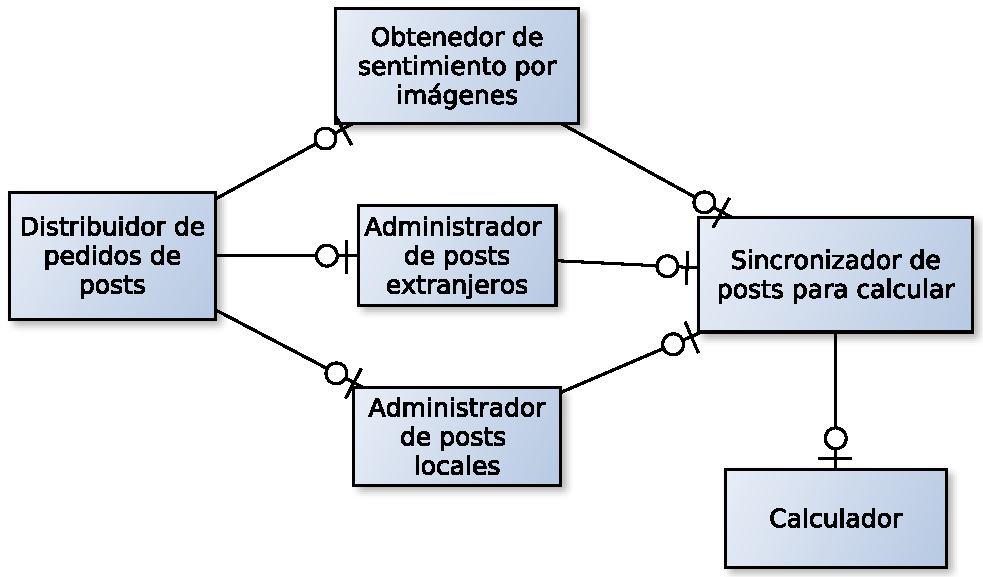
\includegraphics[width=0.7\textwidth]{graph/sincro.pdf}
%\caption{Post Filterer}
\end{figure}

El sincronizador recibe datos de tres fuentes distintas: posts locales, es decir, del área correspondiente al nodo que está ejecutando el pedido; posts extranjeros, que fueron procesados y calificados en los nodos de otras áreas, y sentimiento por imágenes, que proviene del sistema externo y trae sentimientos, pero no mensajes. Todos esos datos deben reunirse para cada pedido. Es posible sincronizar todos los datos del mismo pedido gracias a las etiquetas que se aplican al principio del flujo del sistema, las cuales identificana quién pertenece cada dato. Cuando las tres fuentes comunican que ya enviaron todos los datos posibles para un pedido determinado, el sincronizador los envía al calculador para que los procese.

\subsection{Visualizador de resultados}

\begin{figure}[H]
\centering
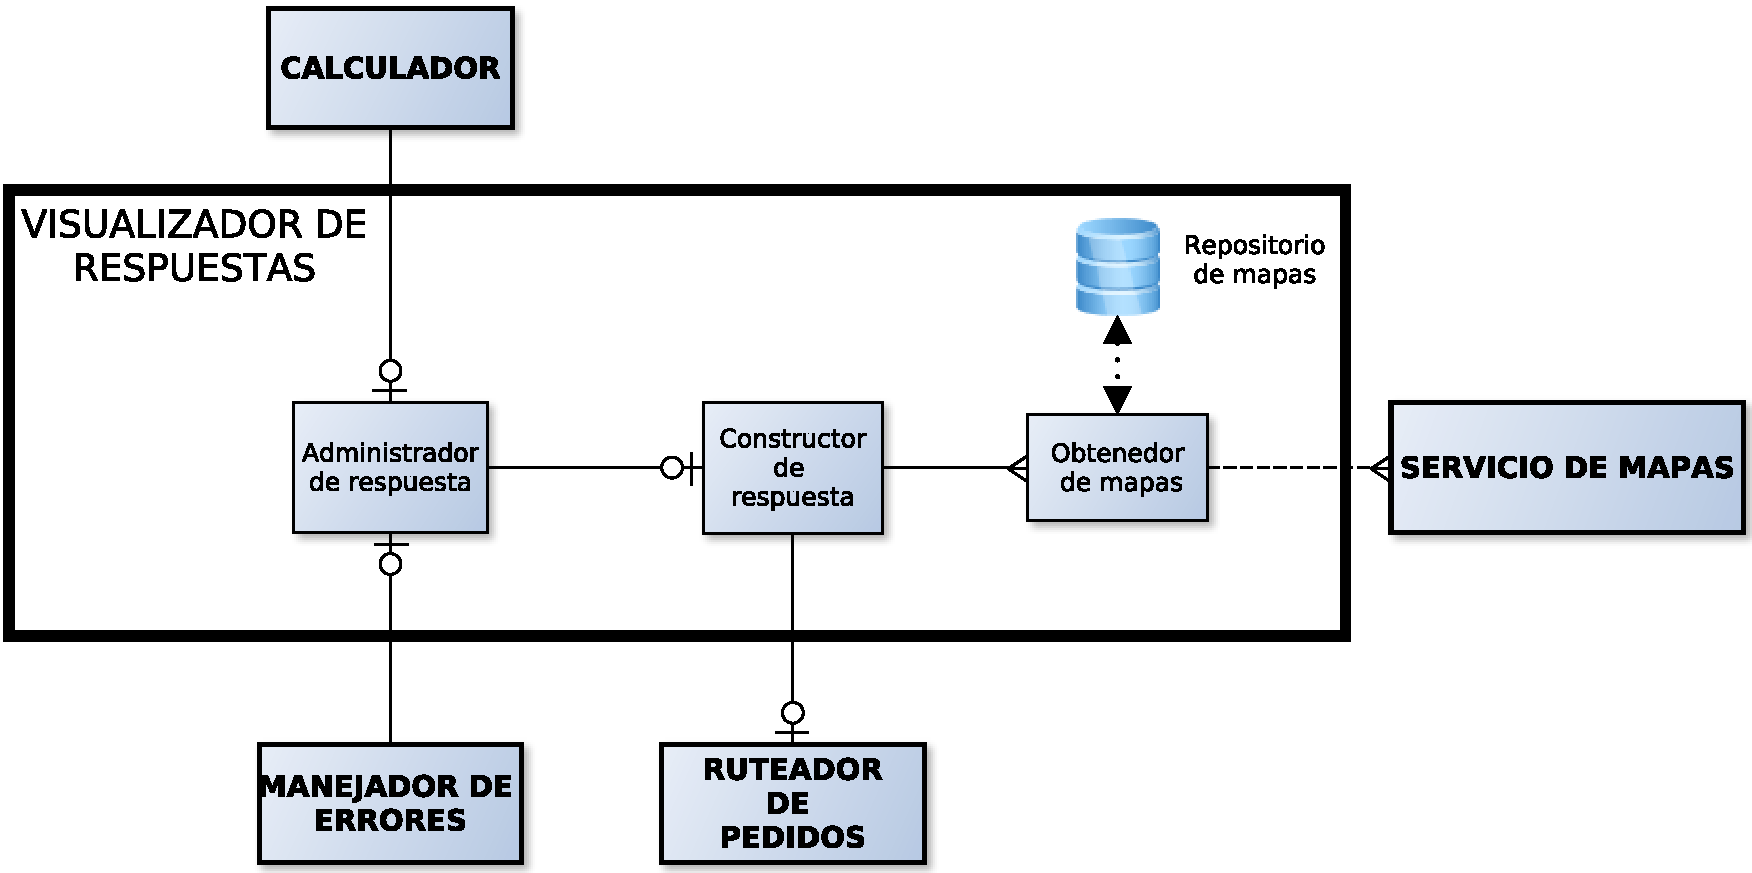
\includegraphics[width=\textwidth]{graph/visualizador.pdf}
%\caption{Post Filterer}
\end{figure}

El visualizador de resultados se encarga de darle formato a la respuesta que recibirá el cliente, ya sea un resultado de rating o popularidad, un mensaje de error, debido a que la consulta del cliente fue invalidada en algún momento por el procesador de pedidos, o un mapa donde se visualizan los resultados. Para ello, el visualizador cuenta con un administrador cola de resultados. A medida que se van desencolando dichos mensajes, estos son comunicados al constructor de respuesta, que se encarga de darles el formato correspondiente según la UI que se esté utilizando o, por ejemplo, un correcto mensaje de error. También se puede comunicar con el obtenedor de mapas, quien provee de un mapa, ya sea buscándolo en repositorio local o en algún servicio de internet como Google Maps. Tal vez este repositorio no sea de tanta utilidad debido al cambio constante del rating, pero tal afirmación habría que hacerla luego de un análisis estadístico de los pedidos de los usuarios. Por último, se envía la respuesta al ruteador de pedidos quien la comunicará al usuario.
